

%%%%%%%%%%%%%%%% arm kinematics %%%%%%%%%%%%%%

\begin{figure}[H]
    \centering
    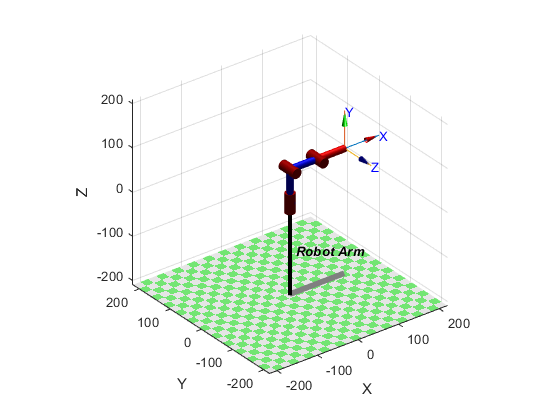
\includegraphics[width=0.6\textwidth]{chapters/img/robot_arm.png}
    \caption{Placeholder image for the robotic arm?.}
    \label{fig:robotic_manipulator_general}
\end{figure}


\section*{Manipulator Kinematics} %Niklas
Kinematics is what describes the motion of rigid bodies and points in space. 

\subsection*{Backgroud}
\subsection*{Rigid body transformation}
In general any position can be described by translation along three axes and rotation along these same axes. These translations/rotations can be described by a matrix
\begin{equation}
    T = 
    \begin{bmatrix}
        R & d \\
        \bf{0} & 1
    \end{bmatrix}
\end{equation}
where \(R\) is a 3 x 3 rotation matrix and \(d\) a 3 x 1 translation matrix. This implies that any transformation could be characterized by six parameters, three for the translation and three for the rotation. \cite{spong}


\subsection*{Denavit-Hartenberg Convention}
A common approach for selecting the coordinate frames of reference for each joint in a robotic arm is the Denavit-Hartenberg convention. This allows the transformation matrix for each joint to be expressed as
\begin{equation}
    A_i = Rot_{z}(\theta_i) \cdot Trans_{z}(d_i) \cdot Trans_{x}(a_i) \cdot Rot_{z}(\alpha_i)
    \label{eqn:DH-transformation}
\end{equation}
that consists of the four basic transformations
\begin{equation}
    Rot_z(\theta_i) = 
    \begin{bmatrix}
        cos(\theta_i) & -sin(\theta_i) & 0 & 0 \\
        sin(\theta_i) & cos(\theta_i) & 0 & 0 \\
        0 & 0 & 1 & 0 \\
        0 & 0 & 0 & 1
    \end{bmatrix}
\end{equation}
\begin{equation}
    Trans_z(d_i) = 
    \begin{bmatrix}
        1 & 0 & 0 & 0 \\
        0 & 1 & 0 & 0 \\
        0 & 0 & 1 & d_i \\
        0 & 0 & 0 & 1
    \end{bmatrix}
\end{equation}
\begin{equation}
    Trans_x(\alpha_i) = 
    \begin{bmatrix}
        1 & 0 & 0 & \alpha_i \\
        0 & 1 & 0 & 0 \\
        0 & 0 & 1 & 0 \\
        0 & 0 & 0 & 1
    \end{bmatrix}
\end{equation}
\begin{equation}
    Rot_z(\theta_i) = 
    \begin{bmatrix}
        1 & 0 & 0 & 0 \\
        0 & cos(\alpha_i) & -sin(\alpha_i) & 0 \\
        0 & sin(\alpha_i) & cos(\alpha_i) & 0 \\
        0 & 0 & 0 & 1
    \end{bmatrix}.
\end{equation}


Where the parameters \(\theta_i\), \(a_i\), \(d_i\) and \(\alpha_i\), known as DH-parameters, characterize each joint. To allow the transformation for each joint to be represented by only four parameters, compared to the six parameters that is required in general, there are some restrictions on how the coordinate frames can be chosen. To comply with the DH-convention, the following must be satisfied.
\begin{itemize}
    \item The axis \(x_{1}\) is perpendicular to the axis \(z_0\)
    \item The axis \(x_{1}\) intersects the axis \(z_0\)
\end{itemize}
where it is assumed that two frames are given, frame 0 and frame 1, and the transformation from equation \ref{eqn:DH-transformation} transforms a coordinate from frame 1 into a coordinate in frame 0.\cite{spong}



\subsection*{Kinematic Chain} %A1*A2*...
A robotic manipulator can be described by a set of joints with links between them where a homogeneous transformation matrix \(A_i\) that describes the transformation with respect to the previous joint exists for each joint. This means that a transformation that describes the position and orientation of joint \(j\) with respect to a joint \(i\) to a can be found by a transformation matrix \cite{spong}
\begin{equation}
    \begin{cases}
        T_j^i = A_{i+1}A_{i+2}...A_{j-1}A_{j}, \text{  if \(i < j\) } \\
        T_j^i = I, \text{  if \(i = j\) } \\
        T_j^i = (T_i^j)^{-1}, \text{  if \(i > j\) }
    \end{cases}
    \label{eqn:Kinematic_chain_spong}
\end{equation}



\subsection*{Forward Kinematics}
Forward kinematics is the problem of finding the position and orientation of the end effector.

Since a manipulator can be seen as a kinematic chain the problem of finding the position and orientation of the end effector can be solved by finding the transformation matrices in equation \ref{eqn:Kinematic_chain_spong}.



\subsection*{Inverse Kinematics}
The problem of finding the joint states required for achieving a desired pose is called inverse kinematics. For some simple kinematic chains an analytical solution exists, but in general a numerical approach might be required. 

%we have for joints, three needed for position. geometric approach for finding the position. then joint for is used to control the pitch of the EOF





\subsection*{Workspace}
A robotic manipulator will not be able to reach all points in space since it has a fixed size. It will not even be able to reach all mathematically reachable points since each joint (usually) have some restrictions on how it can rotate/translate. The physically reachable space is defined as the workspace of the manipulator. %source might be needed here
\\




%%%%%%%%%%%%%%%%%%%%%%%%%%%%%%%%%%%%%%%%%%%%%%%%%%%%%%%%%%%%%%%%
%%%%%%%%%%%%%% Kinematics Implementation %%%%%%%%%%%%%%%%%%%%%%%
%%%%%%%%%%%%%%%%%%%%%%%%%%%%%%%%%%%%%%%%%%%%%%%%%%%%%%%%%%%%%%%%
\subsection*{Implementation}

\subsection*{Denavit-Hartenberg Convention}
In table \ref{tab:DH-table} the DH-parameters that was used for the robotic manipulator, seen in figure \ref{fig:robotic_manipulator_general}, are listed.
\begin{table}[H]
    \centering
    \caption{The Denavit-Hartenberg parameters used for the robotic manipulator.}
    \begin{tabular}{c | c c c c c}
        \(i\) & \(\theta_i\) [rad] & \(d_i\) [mm] & \(a_i\) [mm] & \(\alpha_i\) [rad] \\
        \hline
        \(1\) & \(\theta_1\) & \(75\) & \(0\) & \(\pi / 2\) \\
        \(2\) & \(\theta_2\) & \(0\) & \(67.5\) & \(0\) \\
        \(3\) & \(\theta_3\) & \(0\) & \(67.5\) & \(0\) \\
        \(4\) & \(\theta_4\) & \(0\) & \(65\) & \(0\) \\
    \end{tabular}
    \label{tab:DH-table}
\end{table}



\subsection*{Forward Kinematics}
The transformation matrices from equation \ref{eqn:DH-transformation} for each joint can be multiplied together
\begin{equation}
    T_{end} = A_1 \cdot A_2 \cdot A_3 \cdot A_4
\end{equation}
where \(A_1\) - \(A_4\) are calculated from equation \ref{eqn:DH-transformation} to find the pose \(T_{end}\) of the end effector and thereby solving the forward kinematic problem.


\subsection*{Inverse Kinematics}
To solve the inverse kinematics for the position of a three joint manipulator a geometric method can be used to find an analytical solution. The required angles to achieve a desired position \((x_d, y_d, z_d)\) in an elbow-up configuration are \cite{Lec14_mit_Manipulation}

\begin{equation}
    \begin{cases}
        \theta_1 = Atan(x, y) \\
        \theta_3 = Atan(D, +\sqrt{1 - D^2}) \\
        \theta_2 = Atan(\sqrt{x_d^2 + y_d^2}, z_d - d_1) \\- Atan(a_2 + a_3 \cdot D, a_3 \cdot \sqrt{1 - D^2}) %fix
    \end{cases}
\end{equation}
where \(Atan(x, y)\) is the two argument arctangent function \cite{inverse_tangent_wolfram} and 
\begin{equation}
    D = \frac{x_d^2 + y_d^2 + (z_d - d_1)^2 - a_2^2 - a_3^2}{2 a_2 a_3}
\end{equation}
and \(a_2\), \(a_3\), and \(d_1\)   are the corresponding DH-parameters.



\subsection*{Workspace}
The robotic manipulator seen in figure \ref{fig:robotic_manipulator_general} has the following limitations for the first three joints
\begin{equation}
    \begin{cases}
        -100^\circ < \theta_1 < 100^\circ \\
        -100^\circ < \theta_2 < 100^\circ \\
        -100^\circ < \theta_3 < 100^\circ 
    \end{cases}
    \label{eqn:workspace_limits_angles}
\end{equation}
and a simulated 2D slice of the workspace can be seen in figure \ref{fig:workspace_simulated}. The full workspace can be formed by rotating this 2D slice around the z-axis according to the limitations on \(\theta_1\) from equation \ref{eqn:workspace_limits_angles}.


\begin{figure}[H]
    \centering
    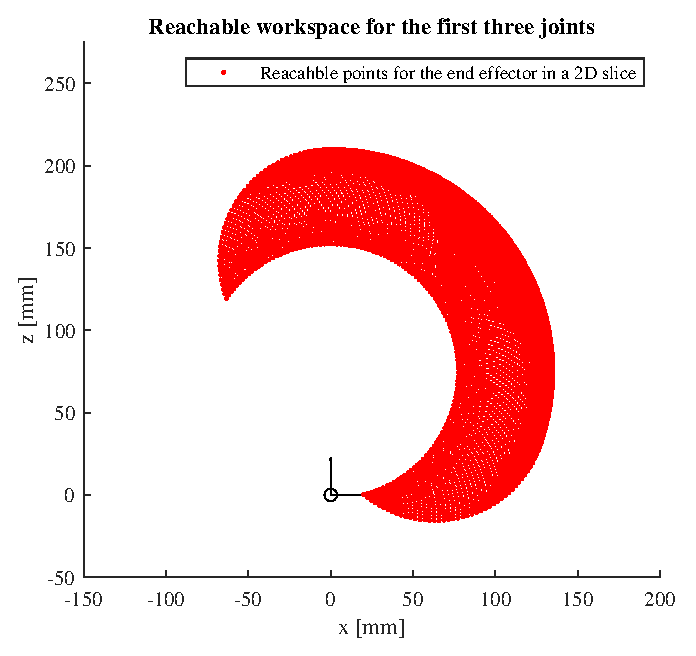
\includegraphics[width=0.45\textwidth]{chapters/img/workspace.eps}
    \caption{A simulated 2D slice of the workspace for the three jointed manipulator.}
    \label{fig:workspace_simulated}
\end{figure}





%%%%%%%%%%%%%%%% arm kinematics end %%%%%%%%%%%%%%













\section*{Base}

The motors will be connected to tracks on the robot and can therefore be modelled as two wheels connected with a rod, as seen in figure \ref{fig:base_math_model}.\\ 
Deriving a mathematical model is straight forward if we can read the encoders from the motors. From the encoders we would be able to get both the length the robot has traveled and more importantly the individual speed each motor rotates with. The speed for the individual motor is given by: 

\begin{equation}
    v_m=\frac{2\pi r_{wh}/N_{enc}}{\Delta t}
    \label{eq:base_system_eq1}
\end{equation}

\noindent Where $N_{enc}$ is the number of encoders on the motor, $r_{wh}$ is the radius of the driving wheel and thickness of the track and $\Delta t$ is the time between the previous encoder reading and the most recent one. By doing this for both the left and right motor we can find how fast the robot is moving along the line by:

\begin{equation}
    \overline{v}= \frac{v_L+v_R}{2}(-\cos \theta \hat{i}+ \sin \theta \Hat{j})
\end{equation}

\noindent Where the $y$-axis parallel to the line. In a similar fashion the angular velocity can be calculated using:

\begin{equation}
    \Dot{\theta} = \frac{v_R-v_L}{2r_{b}}
    \label{eq:base_system_eq2}
\end{equation}

\noindent Where $r_{b}$ is the distance from the center of the base to the wheels. From this and figure \ref{fig:base_math_model} it's easy to see that the change of angle then becomes:

\begin{equation}
    \theta = sin^{-1}\left(\frac{V_L-V_R}{2r_{b}}t\right)
\end{equation}

\begin{figure}[H]
    \centering
    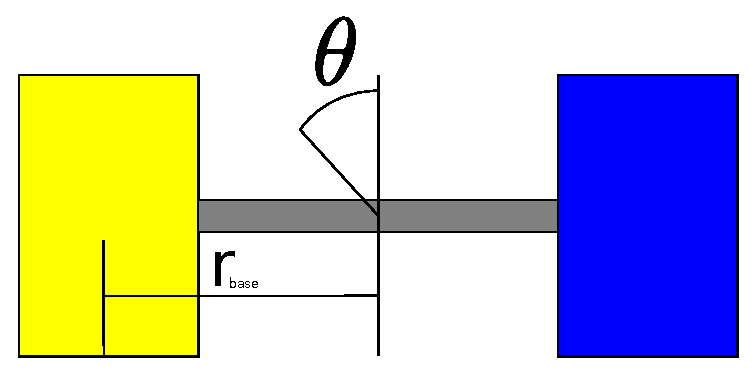
\includegraphics[width=0.7\textwidth]{base_math_model.eps}
    \caption{Modelling of the base as two wheels connected with a rod, where $\theta$ is the angle to the line}
    \label{fig:base_math_model}
\end{figure}

Given the use of small-angles approximation\footnote{Which will be assumed since the robot will be operating on a grid with hard coded functions for turning at QR-codes}, the angular velocity can be written as:

\begin{equation}
    \theta = \frac{V_L-V_R}{2r_{b}}t
\end{equation}


\noindent Using equations \eqref{eq:base_system_eq1}-\eqref{eq:base_system_eq2} a system can be built for simulations in matlab, using rate of change and max/min value limiters for simulations of the motors physical restrictions.

%%%%%%%%%%%%%%%%%%%%%%%%%%%%%%%%%


\section*{Camera vision and calibration}
In this section it is outlined the theory behind the camera vision system. 
How points in a 3D-space are projected on a 2D-plane, calibration and distortion correction. 
\subsection*{Camera model}
\subsection*{Distortion}
